\section{Schematic und PCB}
\subsection{ESP32-S3}
Wie bereits zuvor besprochen, soll eine eigenes PCB entwickelt werden, um alle Geräte darauf unterzubringen.
Im Zentrum der Platine wird sich das \textbf{ESP32-S-WROOM-1} Modul befinden. Es läuft mit bis zu 240 MHz und ist mit einem 2,4 GHz-Transceiver ausgestattet,
der potenziell \textcolor{blue}{Bluetooth}- oder \textcolor{blue}{WIFI}-Unterstützung bietet.
Mit 36 verfügbaren GPIO-Pins stehen uns zahlreiche Möglichkeiten für zusätzliche Funktionen offen.

\begin{figure}[ht]
    \centering
    \begin{subfigure}{0.45\textwidth}
        \centering
        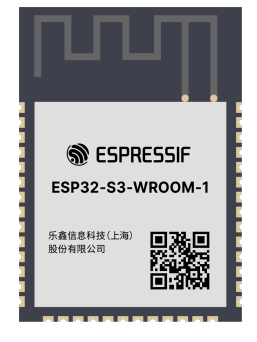
\includegraphics[width=\textwidth]{images/ESP32-S3.png}
        \caption{Top view}
        \label{fig:image1}
    \end{subfigure}
    \hfill
    \begin{subfigure}{0.50\textwidth}
        \centering
        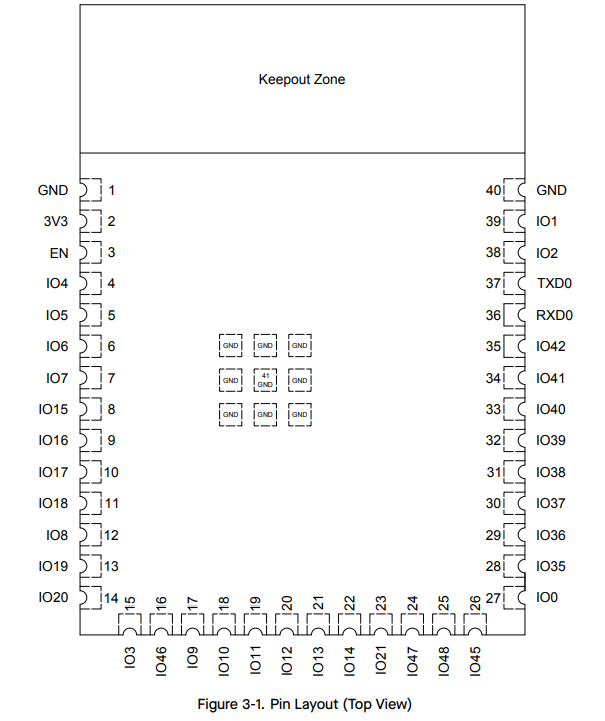
\includegraphics[width=\textwidth]{images/ESP32-S3-schem.png}
        \caption{Schematic}
        \label{fig:image2}
    \end{subfigure}
    \caption{ESP32-S3-WROOM-1}
    \label{fig:both_images}
\end{figure}
\newpage
\subsection{Stromversorgung und Kommunikation}


Zu unserem vorteil, besistz der \textbf{ESP32-S-WROOM-1} native \textbf{USB 2.0} Unterstützung. Diese tatsache ermöglicht
es uns per USB mit dem Modul zu kommunizieren und gleichzeitig die Platine zu versorgen. Um nun dennoch die Vroteile der kompatibilität
von USB-C anstatt USB 2.0 nutzen zu könnnen, sind einige dinge bei der Auslegung zu beachten. Hierbei können wir  die 
\textcolor{red}{CCx (A5,B5)} termination Pins des Steckers nutzen um unseren Stromverbrauch, gemäß der USB-C Spezifikation 
den Host Device bekannt geben ohne einen Powercontroll-IC zu benötigen mit lediglich  10k\si{\ohm} pulldowns zu GND.
Des weiteren nutzen wir weiterhin für die kommunikation die \textbf{USB 2.0} Pins \textcolor{red}{D+, D- (A6,B6,A7,B7)}.

\begin{figure}[h]
    \centering
    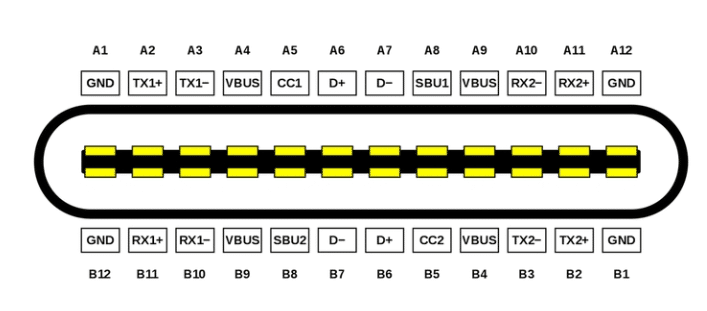
\includegraphics[width=1\linewidth]{images/usbcpinout.png}
    \caption{USB-C Pinout}
    \label{fig:v24}
\end{figure}

\begin{figure}[h]
    \centering
    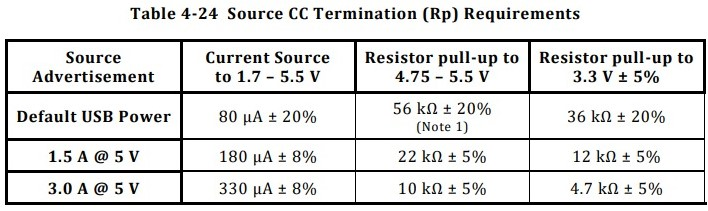
\includegraphics[width=1\linewidth]{images/usbc.png}
    \caption{USB-C Power request}
    \label{fig:v24}
\end{figure}
\newpage
Durch die vorherigen besprochenen methoden kommt folgendes Schematic zustande. 
\begin{figure}[h]
    \centering
    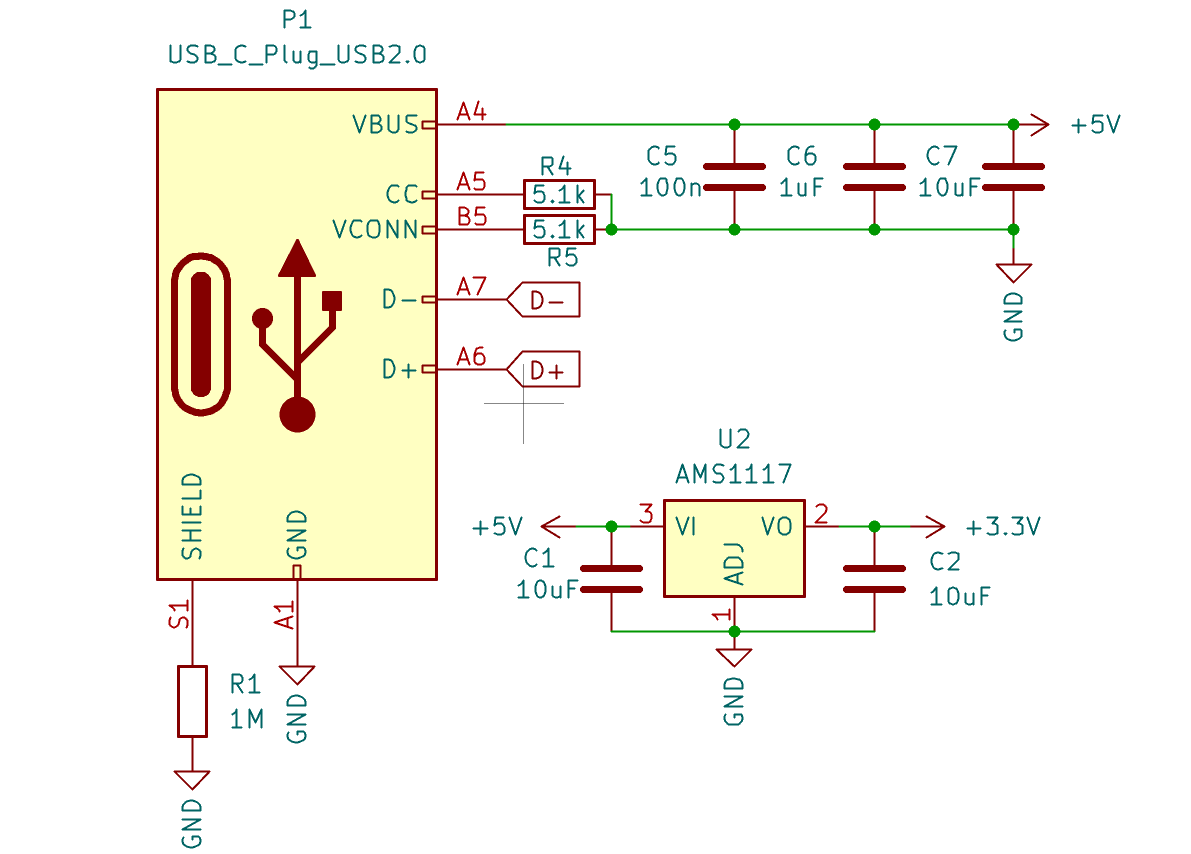
\includegraphics[width=1\linewidth]{images/usbcsch.png}
    \caption{USB-C Schematic}
    \label{fig:v24}
\end{figure}
\\



Zusätzlich müssen wir uns außer die native 5V Spannung von USB-C ebenfalls eine 3.3V versorgungsspannung erzeugen, die den
\textbf{ESP32-S-WROOM-1}, sowie die Sensoren mit Spannung versorgt. Hierfür nutze ich den \textbf{AMS1117} Low-Dopout-Regulator(LDO).
Dieser wandelt die übrige Spannung die in ihnen eingespeißt wird in wärme um, was es ihm erlaubt eine 3.3V Ausgangsspannung zu erzeugen
mit einem Maximal Strom von bis zu 1A, was mehr als genug ist für unseren ESP32 und die restlichen komponennten.

\newpage
\subsection{I$^{2}$C  Busslinie und Sensoren}
Um nun die gewollte funktion der Umgebungserfassung zu gewährleisten sind natürlich Sensoren erforderlich. Die kriterien
nach denen ich diese ausgewählt habe sind wie folgt:\\

$\cdot$ 3.3V Kompatibel\\
$\cdot$ I${^2}$C Kompatibel\\
$\cdot$ günstig und verfügbar als Modul\\\\

Dabei habe ich mich für folgende Komponennten entschieden.

\begin{table}[h]
\centering
\caption{Übersicht der Sensoren und ihrer Funktionen}
\label{tab:sensoren}
\begin{tabular}{>{\raggedright\arraybackslash}p{3cm}>{\raggedright\arraybackslash}p{8cm}}
\toprule
\textbf{Sensor} & \textbf{Funktion} \\
\midrule
BMP390 & Hochpräziser digitaler Luftdrucksensor mit sehr niedrigem Rauschen. Misst den absoluten Luftdruck. Wird häufig für Höhenmessung, Wetterstationen und IoT-Anwendungen verwendet. \\
\addlinespace
INA219AxD & Bidirektionaler Gleichstrom-Messverstärker mit I\textsuperscript{2}C-Schnittstelle. Misst Spannung, Strom und Leistung über einen Shunt-Widerstand. Ideal für Energieverwaltungssysteme. \\
\addlinespace
LM75B & Digitaler Temperatursensor und Thermostat mit I\textsuperscript{2}C-Schnittstelle. Misst Temperaturen von -55°C bis +125°C mit einer Genauigkeit von ±2°C. Einfache Plug-and-Play-Lösung. \\
\addlinespace
SHTC3 & Digitaler Feuchtigkeitssensor mit I\textsuperscript{2}C-Schnittstelle. Bietet hohe Genauigkeit bei niedrigem Stromverbrauch. Ideal für HVAC-Systeme und Wetterüberwachung. \\
\bottomrule
\end{tabular}
\end{table}

\newpage

\begin{figure}[h]
    \centering
    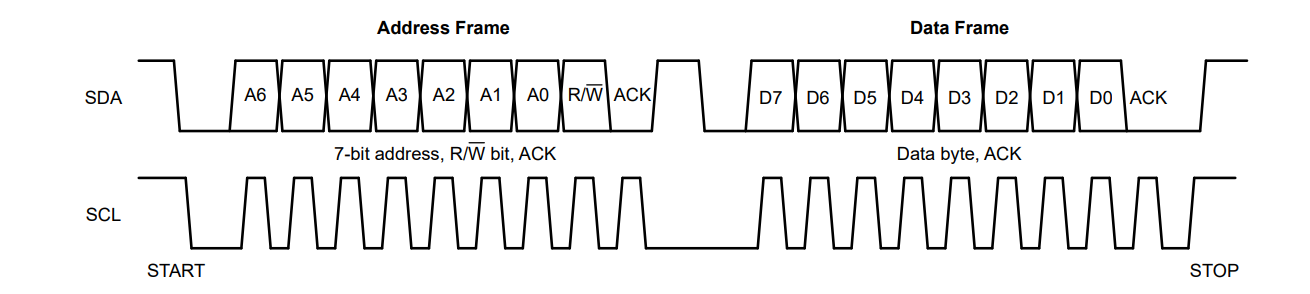
\includegraphics[width=1\linewidth]{images/i2cwork.png}
    \caption{I2C Adress and Data Frames \cite{I2C}}
    \label{fig:v24}
\end{figure}



